\documentclass{beamer}
\usepackage{amsmath,amssymb}
\usetheme{AnnArbor}
\usecolortheme{beaver}

\usepackage{tikz}
\usetikzlibrary{arrows,trees}

\newcommand\m[1]{\mathbb { #1 }}
\newcommand\p[1]{\mathcal{ #1 }}
\newcommand\N{\ensuremath{\m N}}
\let \forces \Vdash

\title{The Set of Arithmetical Sets is not Arithmetical}
\subtitle{(from arithmetical forcing point of view)}
\author{Tom\'a\v s~Jakl}
\institute[KAM MFF]{
    Department of Applied Mathematics (KAM) \\
    Charles University in Prague
}
\date[J\v S KA 2013]{
    Spring School of Algebra \\
    \v Cesk\'y r\'aj, 2013
}

\begin{document}
\frame{\titlepage}

\section{Basic definitions}
\subsection{Language}
\frame{

    \begin{definition}
    Let $\mathfrak L$ denote the first-order language with a constant $\bar n$ for each $n \in \N$, an unary relation `$\cdot \in X$' and function and relation  symbols $+$, $\times$,  $<$, $=$.
    \end{definition}

    \pause
    \begin{definition}
    Let $\varphi$ be a formula of language $\mathfrak L$. We say $\varphi \in
    \Sigma_n$ if $\varphi$ is equivalent to a formula of the form
    \[
        \underbrace{(\exists \vec x_1)(\forall \vec x_2)(\exists \vec x_3)\ldots}_{\leq n}\psi(\vec x_1, \vec x_2, \vec x_3, \ldots)
    \]

    Where formula $\psi$ contains only \emph{bounded} quantifiers. \pause Similarly define $\varphi \in \Pi_n$ for $\varphi$ equivalent to a formula of the form

    \[
        \underbrace{(\forall  \vec x_1)(\exists \vec x_2)(\forall \vec x_3)\ldots}_{\leq n}\psi(\vec x_1, \vec x_2, \vec x_3, \ldots).
    \]

    As a shortcut set $\Delta_n = \Sigma_n \cap \Delta_n$.
    \end{definition}
}

\frame{
    \frametitle{Useful examples}
    \begin{columns}[c]
    \begin{column}{3cm}
        \hspace{0.3cm}
        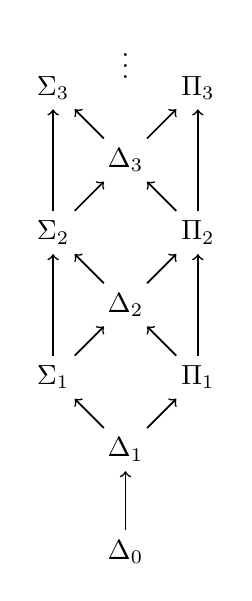
\begin{tikzpicture}[->, node distance=1.3cm, semithick]
            \node (Delta0) {$\Delta_0$};
            \node (Delta1) [above of=Delta0]       {$\Delta_1$};
            \node (Sigma1) [above left of=Delta1]  {$\Sigma_1$};
            \node (Pi1)    [above right of=Delta1] {$\Pi_1$};
            \node (Delta2) [above left of=Pi1]     {$\Delta_2$};
            \node (Sigma2) [above left of=Delta2]  {$\Sigma_2$};
            \node (Pi2)    [above right of=Delta2] {$\Pi_2$};
            \node (Delta3) [above left of=Pi2]     {$\Delta_3$};
            \node (Sigma3) [above left of=Delta3]  {$\Sigma_3$};
            \node (Pi3)    [above right of=Delta3] {$\Pi_3$};
            \node (dots)   [above of=Delta3]       {\vdots};
            \draw (Delta0) -> (Delta1);
            \draw (Delta1) -> (Sigma1);
            \draw (Delta1) -> (Pi1);
            \draw (Sigma1) -> (Sigma2);
            \draw (Sigma1) -> (Delta2);
            \draw (Pi1)    -> (Pi2);
            \draw (Pi1)    -> (Delta2);
            \draw (Delta2) -> (Sigma2);
            \draw (Delta2) -> (Pi2);
            \draw (Sigma2) -> (Sigma3);
            \draw (Sigma2) -> (Delta3);
            \draw (Pi2)    -> (Pi3);
            \draw (Pi2)    -> (Delta3);
            \draw (Delta3) -> (Sigma3);
            \draw (Delta3) -> (Pi3);
        \end{tikzpicture}
    \end{column}
    \begin{column}{9.0cm}
        \begin{itemize}
            \pause
            \item There exist $\Sigma_0$ formulas $\mbox{Concat}(\sigma_1,\sigma_2,\sigma_3)$ and $\mbox{Pref}(\sigma_1,\sigma_2)$ such that:
                \begin{align*}
                    \mbox{Concat}(\sigma_1,\sigma_2,\sigma_3) \text{ is true} & \iff \sigma_1\mathbin{\raisebox{1ex}{\scalebox{.7}{$\frown$}}}\sigma_2 = \sigma_3 \\
                    \mbox{Pref}(\sigma_1,\sigma_2) \text{ is true} & \iff \sigma_1 \subseteq \sigma_2
                \end{align*}

                For $\sigma_1, \sigma_2, \sigma_3 \in \{0,1\}^*$.
            \pause
            \item Working with formulas is in $\Sigma_0$ (G\" odel numbering, decomposing, \dots).
        \end{itemize}
    \end{column}
    \end{columns}
}

\subsection{The Truth and Forcing}

\frame[<+->]{
    \frametitle{The Truth}

    \begin{definition}
        Given a formula $\varphi$ of $\mathfrak L$, $\varphi$ \emph{is true for} $A \subseteq \N$ ($A \models \varphi$) is inductively defined as follows:

    \vspace{0.3em}
    \begin{tabular}{l c l}
    $A \models \varphi \text{ is atomic without `} \cdot \in X$' & $\iff$ & $\varphi$ is true in \N \\
        $A \models \bar n \in X$ & $\iff$ & $n \in A$ \\
        $A \models \neg \psi$ & $\iff$ & not $A \models \psi$ \\
        $A \models \psi_0 \lor \psi_1$ & $\iff$ &  $A \models \psi_0$ or $A \models \psi_1$ \\
        $A \models (\exists x)\psi(x)$ & $\iff$ &for some $n\in\N$, $A \models \psi(\bar{n})$. \\
        \end{tabular}
    \end{definition}

    \begin{block}{Remark}
    Missing conjunction and universal quantifier can be defined by
    \begin{align*}
        \psi_1 \land \psi_2 & \equiv \neg (\neg\psi_1 \lor \neg\psi_2) \\
        (\forall x)\psi(x) & \equiv \neg (\forall x) \neg \psi(x).
    \end{align*}
    \end{block}
}

\frame{
    \frametitle{Forcing}
    \begin{definition}
        Given a formula $\varphi$ of $\mathfrak L$ and $\sigma \in \{0,1\}^*$, $\sigma$ \emph{forces}
        $\varphi$ ($\sigma \forces \varphi$) is inductively defined as follows:

        \vspace{0.3em}
        \begin{tabular}{l c l}
            $\sigma \forces \varphi \text{ is atomic without `} \cdot \in X$' & $\iff$ & $\varphi$ is true in \N \\
            $\sigma \forces \bar n \in X$ & $\iff$ & $\sigma(n) = 1$ \\
            $\sigma \forces \neg \psi$ & $\iff$ & $(\forall \tau \supseteq \sigma)(\tau \not\forces \psi$) \\
            $\sigma \forces \psi_0 \lor \psi_1$ & $\iff$ &  $\sigma \forces \psi_0$ or $\sigma \forces \psi_1$ \\
            $\sigma \forces (\exists x)\psi(x)$ & $\iff$ &for some $n\in\N$, $\sigma \forces \psi(\bar{n})$. \\
        \end{tabular}
    \end{definition}

    \pause
    \begin{block}{Properties}
        \begin{itemize}
            \item \emph{Monotonicity:} if $\sigma \forces \varphi$ and $\tau \supseteq \sigma$, then $\tau \forces \varphi$.
            \item \emph{Consistency:} not ($\sigma \forces \varphi$ and $\sigma \forces \neg\varphi$).
            \item \emph{Quasi-completeness:} $(\forall \sigma)(\exists \tau \supseteq \sigma)(\tau \forces \varphi \text{ or } \tau \forces \neg\varphi)$.
        \end{itemize}
    \end{block}
}

\frame{
    \begin{examples}
    \begin{itemize}
        \item $\sigma \forces \bar n \not\in X$ if and only if $\sigma(n) = 0$.
        \item For $\varphi \equiv (\forall x)(x \in X)$, $\N \models \varphi$ but $\sigma \forces \varphi$ for no $\sigma \in \{0,1\}^*$.
    \end{itemize}
    \end{examples}

    \pause
    \begin{block}{Remark}
        Behaviour of universal quantification and conjuction differs for truth and for forcing.
    \end{block}

    \vspace{1em}
    Compare
    \begin{align*}
        A \models \psi_1 \land \psi_2 & \iff A \models \psi_1 \text{ and } A \models \psi_2 \\
        A \models (\forall x)\psi(x) & \iff \text{for all $n$, }  A \models \psi(\bar{n})
    \end{align*}

    with
    \begin{align*}
        \sigma \forces \psi_1 \land \psi_2 & \iff (\forall \tau \supseteq \sigma) (\exists \tau_1, \tau_2 \supseteq \tau) (\tau_1 \forces \psi_1 \text{ and } \tau_2 \forces \psi_2) \\
        \sigma \forces (\forall x)\psi(x) & \iff (\forall n)(\forall \tau \supseteq \sigma)(\tau_1 \forces \psi(\bar{n})).
    \end{align*}
}

\subsection{Genericity}

\frame{
    \begin{definition}
        For given $A \subseteq \N$ we say $A$ \emph{forces} $\varphi$ ($A \forces \varphi$) if for some finite $\sigma \subseteq A$, $\sigma \forces \varphi$.
    \end{definition}

    \pause
    \begin{block}{Remarks}
        \begin{itemize}
            \item \emph{Consistency}: not ($A \forces \varphi$ and $A \forces \neg\varphi$).

            \item There exists a $A \subseteq \N$ and sentence $\varphi$ such that $A \forces \varphi$ but $A \models \neg\varphi$.
        \end{itemize}
    \end{block}

    \pause
    \begin{definition}
        \begin{itemize}
        \item $A$ is \emph{$n$-generic} if for all sentences $\varphi \in \Sigma_n$ either $A \forces \varphi$ or $A \forces \neg\varphi$.
        \item $A$ is \emph{$\omega$-generic} if the same happens for all sentences of $\mathfrak L$.
        \end{itemize}
    \end{definition}
}

\frame{
    \begin{lemma}[Forcing = Truth for generics sets]
        $A$ is $n$-generic iff for any sentence $\varphi \in \Sigma_n \cup \Pi_n$, $A \models \varphi \iff A \forces \varphi$.
        Consequently the same holds for $A$ $\omega$-generic and $\varphi$ arbitrary.
    \end{lemma}

    \pause
    \begin{proof}
        Suppose $A$ is $n$-generic and proceed by induction on complexity of $\varphi$. Definitions of $\forces$ and $\models$ differ on negation part only. Let $\varphi \equiv \neg\psi$, then:
        \begin{align*}
             & A \models \neg \psi & \\
        \iff & A \not \models \psi & \\
        \iff & A \not\forces \psi  & \text{ (by induction)}\\
        \iff & A \forces \neg\psi  & \text{ (genericity of $A$).}
        \end{align*}

        \pause
        For converse take any $\varphi \in \Sigma_n$. Either $A \models \varphi$ or $A \models \neg\varphi$ holds and so either $A \forces \varphi$ or $A \forces \neg\varphi$ holds.
    \end{proof}
}

\subsection{Definability of $\forces$}

\frame{
    \begin{lemma}[Definability of forcing]
        The relation ``$\sigma \forces \varphi$'' is defined by a $\Sigma_{n+1}$ formula in variables: $\varphi \in \Sigma_n$, $\sigma \in \{0,1\}^*$.
    \end{lemma}

    \pause
    \begin{proof}
    By induction on complexity of $\varphi$. In a decision process for $\sigma \forces \varphi$ are quantifiers introduced in the following cases only:

    \begin{itemize}
    \item $\varphi \equiv (\exists x)\psi(x)$: $\sigma \forces \varphi$ iff $(\exists n)(\sigma \forces \psi(\bar{n}))$.
    \item $\varphi \equiv \neg\psi$: $\sigma \forces \varphi$ iff $(\forall \tau \supseteq \sigma) (\tau \not\forces \psi)$.
    \end{itemize}
    \end{proof}
}


\section{Demonstration of the method}

\frame{
    \begin{definition}
        A set $A \subseteq \N$ \emph{is defined by} a formula $\varphi$ if $n \in A \iff \emptyset \models \varphi(\bar{n})$. A set $A$ is said to be \emph{arithmetical} if it is defined by some formula of $\mathfrak L$.
    \end{definition}

    \pause
    \begin{theorem}
        There is a $n$-generic set defined by $\Sigma_{n+1}$ formula.
    \end{theorem}
    \only<1-2>{\vspace{13.1em}}
    \only<3>{\begin{proof}[Proof idea.]
        \begin{enumerate}
            \item We have $\Sigma_0$ enumeration of $\Sigma_n$ sentences: $\psi_0, \psi_1, \dots$.
            \item For each $\psi_i$ we $\Sigma_{n+1}$-find a string $\sigma_i$ extending $\sigma_{i-1}$ such that $\sigma_i \forces \psi_i$ or $\sigma_i \forces \neg\psi_i$.
            \item $\bigcup_i \sigma_i$ is a characteristic function of a $n$-generic.
        \end{enumerate}
    \end{proof}
    \vspace{3.2em}}
    \only<4>{\begin{proof}
        Define a formula $\varphi(x)$ equivalent to
        \begin{align*}
            (\exists \vec \sigma) & ((\forall i \in \{1, \ldots, x\}) \text{ minimal $\sigma_i$ s.t.}\\
            & (\sigma_i \forces \psi_i \text{ or } \sigma_i \forces \neg\psi_i) \text{ and }\\
            & (\sigma_i \supseteq \sigma_{i-1}) \text{ and } (|\sigma_i| \geq i)) \\
        \text{ and } & (\sigma_x(x) = 1).
        \end{align*}

        Then the set defined by $\varphi(x)$ is $n$-generic.
    \end{proof}}
}

\subsection{Topological nature of forcing}

\frame{
    \frametitle{$2^\omega$ as infinite binary tree}
    \begin{columns}
    \begin{column}{8cm}
    \begin{block}{Properties of $2^\omega$}
    \begin{itemize}
        \item Compact hence locally compact.
        \item The sets $[\sigma] = \{ A \subseteq \N: A \supseteq \sigma \}$ form a basis of product topology.
        \item Hausdorff.
    \end{itemize}
    \end{block}

    % \vspace{1.5em}
    % \only<2>{
    % The proof went exactly the same way as the proof of Baire category
    % theorem (theorem which says: in a complete metric/locally compact
    % Hausdorff space a countable intersection of dense sets is dense).
    % }


    \end{column}
    \begin{column}{4cm}
    \hspace{0.3cm}
    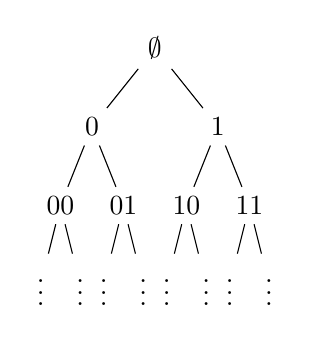
\begin{tikzpicture}[level distance=1.0cm,
        level 1/.style={sibling distance=1.6cm},
        level 2/.style={sibling distance=0.8cm},
        level 3/.style={sibling distance=0.5cm}]
        \node {$\emptyset$}
            child {node {0}
                child {node {00}
                    child {node {\vdots}}
                    child {node {\vdots}}
                }
                child {node {01}
                    child {node {\vdots}}
                    child {node {\vdots}}
                }
            }
            child {node {1}
                child {node {10}
                    child {node {\vdots}}
                    child {node {\vdots}}
                }
                child {node {11}
                    child {node {\vdots}}
                    child {node {\vdots}}
                }
            };
    \end{tikzpicture}
    \end{column}
    \end{columns}
}

\frame{
    \begin{lemma}
        The set $\p O_\varphi = \{A \subseteq \N : A \forces \varphi \text { or } A \forces
        \neg\varphi\}$ is open and dense in $2^\omega$.
    \end{lemma}

    \pause
    \begin{proof}
        \begin{itemize}
            \item The set $\p O_\varphi$ is open since it is an union of all $[\sigma]$ such that $\sigma \forces \varphi$ or $\sigma \forces \neg\varphi$.

            \pause
            \item The set $\p O_\varphi$ is dense. Indeed, take any $\sigma$:

            \begin{itemize}
                \item If $(\forall \tau \supseteq \sigma) (\tau \not\forces \varphi)$ then $\sigma \forces \neg\varphi$.

                \item If $(\exists \tau \supseteq \sigma) (\tau \forces \varphi)$ then $\p O_\varphi \cap [\sigma] \neq \emptyset$ since $[\tau] \subseteq [\sigma]$.
            \end{itemize}
        \end{itemize}
    \end{proof}
}

\frame{
    \begin{definition}
        \begin{itemize}
        \item A subset of topological space is called \emph{meager} if it is a countable union of nowhere dense sets (sets $S$ with $\overline{S}^o = \emptyset$).

        \pause
        \item A subset of topological space is called \emph{comeager} if it is not meager. In other words it contains a countable intersection of open dense sets.
        \end{itemize}
    \end{definition}

    \pause
    \begin{lemma}
        There are comeager many $\omega$-generic sets in $2^\omega$.
    \end{lemma}
    \pause
    \begin{proof}
        Since each $\p O_\varphi$ is open and dense the set $\bigcap_{\varphi \in \mathfrak L} O_\varphi$ is comeager in $2^\omega$.
    \end{proof}
}

\subsection{The main theorem}

\frame{
    \begin{theorem}
        The set of arithmetical sets is not arithmetical.
    \end{theorem}

    \pause
    \begin{proof}
        \begin{enumerate}
            \item Suppose not. We have $X \text { arithmetical} \iff X \models \psi$, for some $n$ and some $\psi \in \Sigma_n$.
            \pause
            \item There exists a $n$-generic set $A$, s.t. $A \models \psi$.
            \pause
            \item Since also $A \forces \psi$, $\sigma \forces \psi$ for some finite $\sigma \subset A$.
            \pause
            \item Let $G$ be a $n$-generic set extending $\sigma$ then $G \forces \psi$, so $G \models \psi$ and therefore $G$ is arithmetical.
            \pause
            \item There are comeager many $n$-generic sets extending $\sigma$ but only meager many arithmetical sets. Contradiction.
        \end{enumerate}
    \end{proof}
}

\frame{
    \begin{center}
    \Huge{May the Force be with you!}
    \end{center}
}

\section{References}

\frame{
    \frametitle{References}

    \begin{thebibliography}{10}
    \bibitem{Odi1}
    Odifreddi, Piergiorgio.
    \newblock Forcing and Reducibilities,
    \newblock \emph{The Journal of Symbolic Logic}, Volume 48, Number 2, June 1983.

    \bibitem{Odi2}
    Odifreddi, Piergiorgio.
    \newblock Classical recursion theory: The theory of functions and sets of natural numbers.
    \newblock Vol. 125. North Holland, 1992.
    \end{thebibliography}
}
\end{document}
